\documentclass{article}
\usepackage[utf8]{inputenc}
\setlength{\parindent}{0pt} 
\usepackage{amssymb}
\usepackage{amsmath}
\usepackage{graphicx}
\usepackage{float}
\newcommand{\N}{\mathbb{N}}
\newcommand{\Z}{\mathbb{Z}}
\newcommand{\Q}{\mathbb{Q}}
\newcommand{\R}{\mathbb{R}}
\newcommand{\C}{\mathbb{C}}
\newcommand{\ra}{\longrightarrow}

\title{Homework 1}
\date{}
\author{Julian Lehrer}
\begin{document}
\maketitle
\textbf{Question 1}
Suppose $A$ is both unitary and upper-triangular, that is,
$A^*A=AA^*=UU^{-1}=I$, Therefore, $a_{ij} = 0$ for $i > j$, that is, $A$ is upper triangular. Then we have that $A^*$, the conjugate transpose, is a lower triangular matrix and that $a^*_{ij} = 0$ for $j < i$. Then for the $i$th row, $A^*A_{i, } = \sum_{j=1}^m A_{i, j}A^*_{i, j}=A_{i, i}A^{*}_{i, i }+ 0+...+0 = AA^*{1, }$. So, $A_{i,j}=0$ for $j \neq i$, so $A$ is diagonal. 

\textbf{Question 2.} 
\begin{itemize}
    \item[a.] Let $x$ be such that $Ax =\lambda x$. Then 
    \begin{align*}
        A^{-1}Ax &= A^{-1}\left(\lambda x\right) \\ 
        \implies x = A^{-1}\left(\lambda x\right)\\
        \implies x=A^{-1}\lambda x \\
        \implies A^{-1}x = 1/\lambda x
    \end{align*}
    Therefore, $1/\lambda$ is an eigenvalue of $A^{-1}$. 
    \item[b.] Suppose $AB = \lambda x$. Then $BAB x= B\lambda x$. Since linear maps are associative, we have that $(BA)Bx = \lambda(Bx)$, that is, the eigenvalue of $BA$ is the same as $AB$ with a different eigenvector. Therefore, the eigenvalues of $AB$ and $BA$ are the same 
    \item[c.] Since $A$ is real, $A^* = A^T$, therefore $det(A-\lambda I) = det((A-\lambda I)^T)$. Since the characteristic polynomials are the same, the root (eigenvalues) are the same. 
\end{itemize}

\textbf{Question 3.} 
\begin{itemize}
    \item[a.] We have that $A = A^*$, so $A$ is Hermitian. Then $Ax = \lambda x$. Taking the conjugate transpose of this relation, we have that $x^*A^* = \lambda^*x^*$. Then, $x^*A^*x = \lambda^*x^* x \iff x^*\lambda x = \lambda^*x^*x \iff \lambda x^*x = \lambda^* x^*x \implies \lambda = \lambda^* \implies \lambda \in \R$. 
    \item[b.] Let $Au = \lambda u$ and $Av = \tau v$ where $\lambda \neq \tau$. Then consider 
    \begin{equation*}
        (Au)^* = (\lambda u)^* \implies u^*A^* = \lambda u^* \implies u^*A = \lambda u^*
    \end{equation*}
    Since $A$ is Hermitian. Then multiplying on the right by $v$, we have that 
    \begin{align*}
        u^*Av &= \lambda u^*v \\
        \tau u^*v &= \lambda u^* v\\
        \tau (u, v) &= \lambda (u, v)
    \end{align*} 
    Since $\lambda \neq \tau$, we must have that $(u,v)=0$, that is, the eigenvectors are orthogonal. 
\end{itemize}

\textbf{Question 4.} Proof ($\implies$). Suppose that $A$ is positive-definite and Hermitian. Let $v$ be a a nonzero vector such that $Av = \lambda v$ where $\lambda \in \R$. Then $(Av, v) = (\lambda v)^* v = \lambda v^*v = \lambda \sqrt{(v,v)} > 0$ by assumption. Since $v$ is nonzero, we have that the inner product $(x,x) > 0$ and hence $\lambda > 0$. \\

Proof ($\impliedby$). Suppose $\lambda > 0$, $\lambda \in \Lambda(A)$. Then we have that for $x\neq 0$, $(x, x) > 0 \iff (\lambda x, x) >0\iff (Ax, x) > 0$ therefore $A$ is positive-definite.\\

\textbf{Question 5.} 
\begin{itemize}
    \item[a.] Consider that we have the following two facts: $Ax =\lambda x$ and $(Ax)^*=\left(\lambda x\right)^* \iff x^*A^*=\lambda^* x^*$. Then we have that
    \begin{align*}
        x^* A^* A x &= \lambda^* x^* Ax \\
        x^* \underbrace{A^* A}_{I} x &= \lambda^* \lambda x^* x\\
        x^* x= \lambda^* \lambda x 
    \end{align*} 
    But if $\lambda = a+bi$, then $\lambda^*\lambda = a^2-b^2 = \left| \lambda\right|^2$. Therefore, we must have that $\left| \lambda\right|^2 = 1\implies |\lambda | = 1$ by the equality we derived above. 
    \item[b.] This is false, since have that $\left| A\right|_F = \sqrt{tr(A^*A)} = \sqrt{tr(I)} = n$ where $n$ is the number of columns or rows in the matrix. 
\end{itemize}

\textbf{Question 6.} 
\begin{itemize}
    \item[a.] We have that 
    \begin{align*}
        (Ax)^*x &= (\lambda x)^* x \\
        \iff x^* A^* x &= \lambda^* x^* x\\
        \iff -x^*Ax &= \lambda^*x^*x\\
        \iff -x^*\lambda x &= \lambda^* x^* x \\
        \iff -\lambda (x^*x) &= \lambda^* (x^*x)\\
        \iff -\lambda &= \lambda^*
    \end{align*} 
    Then letting $\lambda = a+bi \iff -\lambda = -a-bi$, we have that $a+bi = -a-bi \iff 2a + bi = -bi$ so $a=0$, and hence $\lambda$ is purely imaginary.
    \item[b.] Suppose $A$ is singular. Then we have that for some $x \neq 0$, $(I-A)x=0$. But this means that $Ix-Ax = 0 \iff Ax = x$, so $x$ is an eigenvector with eigenvalue $1$. This is a contradiction, since the eigenvalues of $A$ are purely imaginary. Hence, $I-A$ is nonsingular
\end{itemize}

\textbf{Question 7.} Suppose that $Av=\lambda v$ for some nonzero vector $v$ such that $\| v \|=1$. Then we have that $\| Av \| = \|\lambda v\| = |\lambda|\|v\|$. Also, since 
\begin{equation*}
    \|A\| = \sup_{\|x\| =1}\|Ax\|
\end{equation*}
We have that 
\begin{align*}
    \sup_{\|x\| = 1}\|Ax\| &\geq \|Av\| \\
    &=\|\lambda x \| = |\lambda|\|x\| = |\lambda|
\end{align*}

Then choose $\lambda = \rho(A)$ since this inequality holds for arbitrary eigenvalues. Therefore, $\|A\| \geq \rho(A)$. \\

\textbf{Question 8. }\\
\begin{itemize}
    \item[a.] First, note that since $\|A\|_2=\sigma_1$, the largest singular value, this implies by definition that $\|A\|_2 = \sqrt{\rho(A^*A)}$ where $\rho(A)$ is the spectral radius of $A$ since $\sigma_i = \sqrt{\lambda_i}$ where $\lambda_i$ is the ith eigenvalue of $A^*A$. Also, we have that 
    \begin{equation*}
        (A^*A) uv^* = vu^*uv^*v^*u = \|u\|_2^2\|v\|_2^2 v^*u
    \end{equation*}
    Therefore
    \begin{align*}
         \sqrt{\rho(A^*A)} = \sqrt{\|u\|_2^2\|v\|_2^2}=\|v\|_2\|u\|_2
    \end{align*} 
    \item[b.] We have that 
    \begin{align*}
        \|A\|_F = \sqrt{\sum_{i=1}^m \sum_{j=1}^n |u_i v_j|^2} = \sqrt{\sum_{i=1}^m |u_i|^2\sum_{j=1}^n |v_j|^2}=\sqrt{\|u\|_2^2\|v\|_2^2}=\|u\|_2 \|v\|_2
    \end{align*} 
\end{itemize}

\textbf{Question 9.} \\
\begin{itemize}
    \item[a.] To show this, we show that $\|Qx\|_2=1$ for any unitary matrix $Q$. By definition, we have that 
    \begin{align*}
        \|Qx\| &= \sqrt{(Qx, Qx)}\\
        &= \sqrt{(Qx)^*Qx}\\
        &=\sqrt{x^*Q^*Qx}=\sqrt{x^*x}=\sqrt{(x, x)} = \|x\|_2
    \end{align*} 
    Therefore, by the associativity of matrix multiplication we have that 
    \begin{equation*}
        \|AQ\|_2 = \sup_{\|x\|_2=1}\|AQx\|_2 =\sup_{\|x\|_2=1}\|A(Qx)\|_2= \sup_{\|x\|_2=1}\|A\|_2 = \|A\|
    \end{equation*}
    \item[b.] We exploit the fact that $\|A\|_F = \sqrt{tr(A^*A)}=\sqrt{tr(AA^*)}$ from lecture. Then, we have that 
    \begin{align*}
        \|AQ\|_F &= \sqrt{tr((AQ)(AQ)^*)}\\
        &=\sqrt{tr(AQQ^*A^*)}=\sqrt{tr(AA^*)}=\|A\|_F
    \end{align*} 
    and 
    \begin{align*}
        \|AQ\|_F &= \sqrt{tr((QA)^*(QA))}\\
        &=\sqrt{tr(A^*Q^*QA)}= \sqrt{tr(A^*A)}=\|A\|_F
    \end{align*}
    And the equality $\|AQ\|_F = \|QA\|_F$ comes from transitivity. 
\end{itemize}

\textbf{Question 10.}
\begin{itemize}
    \item[a.] Lemma: The product of two unitary matrices is unitary. Proof: Let $A, B$ be unitary, so $AA^*=I$ and $BB^*=I$. Then $(AB)^*(AB) = B^*A^*AB = B^*IB = B^*B = I$, so $AB$ is unitary. Now let $A=U_A\Sigma_A V_A^*$ be the SVD of $A$ adn $B=U_B\Sigma_B V_B^*$ be the SVD of $B$. Then $A=(QV_B)\Sigma_B(V_BQ^*)$. But this is also the SVD for $A$, so $\Sigma_A = \Sigma_B$ by the uniqueness of the SVD. Since the singular values are the square roots of the diagonal of $\Sigma_A$ and $\Sigma_B$, and these are equal, the singular values of $A$ and $B$ are equal. 
    \item[b.] Consider $A$ and $-A$. Then 
\end{itemize}

\textbf{Question 11.}
\begin{itemize}
    \item[a.] Since $f$ is differentiable, we have that 
    \begin{equation*}
        \kappa(f)=\frac{\|J(x)\|}{\|f(x)\|/\|x\|}=\frac{\|x\|\|J(x)\|}{\|f(x)\|}
    \end{equation*} 
    We have that $J=[1,1]^T$, and choosing the $\infty$ norm we have that 
    \begin{equation*}
        \kappa(f)=\frac{\max \{ x_1, x2\}}{|x_1+x_2|}
    \end{equation*}
    Therefore, as $x_1, x_2 \ra 0$, $f$ becomes ill conditioned since $\kappa(f)\ra\infty$
    \item[b.] We have that $J(f)=[x_2, x_1]^T$, therefore the $\infty$ norm on $J$ is $\|J\|_\infty = \max\{ x_1, x2\}$. This gives us that the condition number is 
    \begin{equation*}
        \frac{2\max\{ x_1,x_2\}}{|x_2x_1|}
    \end{equation*}
    Therefore, as $x_1 \ra 0$ or $x_2 \ra 0$, $f$ becomes ill conditioned since $\kappa \ra \infty$ as the denominator goes to zero. 
    \item[c.] Here, we have that $f'(x)=9(x-2)^8$, therefore, the condition number is given by 
    \begin{equation*}
        \kappa(f)=\frac{9(x-2)^8|x|}{|x-2|^9}
    \end{equation*} 
    So as $x \ra 2$, $f$ becomes ill conditioned since $k \ra \infty$
\end{itemize}

\textbf{Question 12.}
\begin{itemize}
    \begin{figure}[H]
        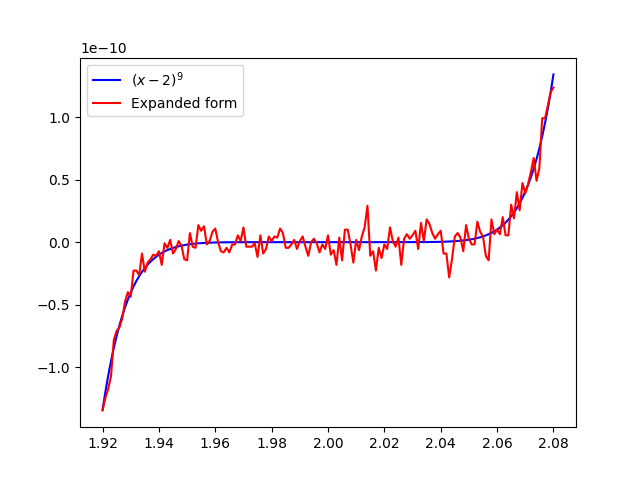
\includegraphics[scale=0.5]{code/question_12.png}        
    \end{figure} 
    \item[a and b] See figure 
    \item[c.] Since we are plotting $f$ around $2$, where the conditioning number goes to $\infty$, we can see the line is perburbed randomly in this domain.
\end{itemize}
\end{document}
